%!TEX root=../../autopilot.tex
\section{Data}
\label{sec:datamodel}

As of v0.5.0, Autopilot uses \href{https://pydantic-docs.helpmanual.io/}{pydantic} to create explicitly typed and schematized data models. Submodules include \texttt{data} abstract \texttt{modeling} tools that define base model types like \texttt{Table}s, \texttt{Group}s, and sets of \texttt{Attributes}. These base modeling classes are then built into a few core data models like subject \texttt{Biography} information, \texttt{Protocol} declaration, and the \texttt{Subject} data model itself that combines them. Modeling classes then have multiple \texttt{interfaces} that can be used to create equivalent objects in other formats, like pytables for hdf5 storage, pandas dataframes for analysis, or exported to Neurodata Without Borders.
\clearpage
For example, consider a simplified version of the \texttt{Biography} model:

\begin{pythoncode*}{label = \texttt{\textbf{data - Biography}}}
from autopilot.data.modeling import Data, Attributes, Field
from typing import Optional, Union|$\tikzmark{typing}$|
from datetime import datetime, timedelta

class Enclosure(Data):|$\tikzmark{dataclass}$|
    """Where does the subject work?"""
    box:  Optional[Union|$\tikzmark{union}$|[str, int]] = Field(
        default=None,
        description="The box this Subject is run in"
    )
    room: Optional[Union[str, int]] = Field(
        default=None,|$\tikzmark{optional}$|
        description="The room number that the animal is run in"|$\tikzmark{description}$|
    )

class Biography(Attributes):|$\tikzmark{attributes}$|
    """Biography of an Experimental Subject"""
    id:  str = Field(...
        description="The indentifying name of this subject."
    )
    dob: datetime|$\tikzmark{datetime}$| = Field(... 
        description="The Subject's date of birth"
    )
    enclosure: Optional[Enclosure]|$\tikzmark{recursive}$| = None

    @property|$\tikzmark{property}$|
    def age(self) -> timedelta:
        """Difference between now and :attr:`.dob`"""
        return datetime.now() - self.dob
\end{pythoncode*}
%
\begin{tikzpicture}[overlay, remember picture, font=\footnotesize]
\draw[<-] (pic cs:typing) ++(0.1,0.1) to[left]%
 ++(5.2,0) --++(0.2,0)%
 node[below right, yshift=8pt, text width=2.4in]{%
Data models use builtin Python type hints. \href{https://docs.python.org/3/library/typing.html}{Type hints} are colon delimited annotations like \mintinline{python}{x:int} that indicate the type (integer, string, etc.) of the variable. Though typically Python does not, Pydantic both validates that a type matches its hint and coerces it to the correct type if possible.};
\draw[<-] (pic cs:union) ++(-0.4,-0.1) --++(0,-0.3)%
 --++(7.3,0) --++(0.2,0)%
  node[below right, yshift=8pt, text width=2.4in]{%
The \texttt{Union} type means that a field can be one of several possible types, in this case the box can be identified with either a string or integer.};
\draw[<-] (pic cs:optional) ++(0,0.1) to[left]%
 ++(7.4,0) --++(0,0.5) --++(0.2,0)%
  node[below right, yshift=8pt, text width=2.4in]{%
Optional fields can have default fields, either a single value like \mintinline{python}{None} or a function that computes a default value like the current date.};
\draw[<-] (pic cs:description) ++(0,0.1) to[left]%
 ++(0.65,0) --++(0,-0.2) --++(0.2,0)%
  node[below right, yshift=8pt, text width=2.4in]{%
Descriptions are stored in the data model schema to make shared data self-documenting, and also used by GUI widgets for tooltips that clarify what fields mean.};
\draw[<-] (pic cs:attributes) ++(0,0.1) to[left]%
 ++(6.3,0) --++(0.2,0)%
  node[below right, yshift=8pt, text width=2.4in]{%
The class that our model inherits from indicates how Autopilot should treat it in a given storage interface. For HDF5 files, subclasses of the Attributes class are stored as node metadata, while subclasses of Table make tables.};
\draw[<-] (pic cs:datetime) ++(-0.6,0.2) --++(0,0.2)%
 --++(8.62,0) --++(0.2,0)%
  node[below right, yshift=8pt, text width=2.4in]{%
Autopilot's format interfaces define mappings from nonstandard types to types supported by the format. For HDF5 files, \href{https://docs.python.org/3/library/datetime.html\#datetime-objects}{datetime} objects are converted to ISO 8601 formatted strings};
\draw[<-] (pic cs:recursive) ++(-1,-0.1) --++(0,-0.2)%
 --++(6.3,0) --++(0,0.5) --++(0.2,0)%
  node[below right, yshift=8pt, text width=2.4in]{%
Data models can be recursive, or use other models as types for their own fields. In this case the subject's Enclosure can be optionally specified in its Biography.};
\draw[<-] (pic cs:property) ++(0.1,0.1) to[left]%
 ++(8.55,0) --++(0,-0.2) --++(0.2,0)%
  node[below right, yshift=8pt, text width=2.4in]{%
Properties are model fields that are automatically computed based on the values of other fields. The age of the animal can be accessed like a normal instance attribute that returns a \href{https://docs.python.org/3/library/datetime.html\#timedelta-objects}{timedelta} object.};
\end{tikzpicture}%
%
The presence and location of the biography information is in turn explicitly specified by the \texttt{Subject\_Structure} data model. A new subject could then be created with a biography like this, storing it in the HDF5 file and made accessible through the Subject interface:

\begin{pythoncode*}{label = \texttt{\textbf{data - New Subject}}}
from autopilot.data import Subject|$\tikzmark{subject}$|
from autopilot.data.models import Biography, Enclosure|$\tikzmark{modelmodule}$|

bio = Biography(
    id="my_subject",
    dob="2022-01-01T00:00:00",|$\tikzmark{coercion}$|
    enclosure=Enclosure(box=100, room="Building 200")
)
sub = Subject.new(bio)
assert sub.info == bio|$\tikzmark{samebio}$|
\end{pythoncode*}
\begin{tikzpicture}[overlay, remember picture, font=\footnotesize]
\draw[<-] (pic cs:subject) ++(0.1,0.1) to[left]%
 ++(5.2,0) --++(0,0.5) --++(0.2,0)%
 node[below right, yshift=8pt, text width=2.4in]{%
The \texttt{Subject} class is the primary means by which Autopilot stores, organizes, and interacts with data.};
\draw[<-] (pic cs:modelmodule) ++(0.1,0.1) to[left]%
 ++(2,0) --++(0.2,0)%
 node[below right, yshift=8pt, text width=2.4in]{%
Several basic models are built into Autopilot, and in future versions it will be possible to extend and replace these models with plugins, making storage formats fully customizable while still being explicit and understandable.};
\draw[<-] (pic cs:coercion) ++(0.1,0.1) to[left]%
 ++(5.8,0) --++(0.2,0)%
 node[below right, yshift=8pt, text width=2.4in]{%
If we don't give the type specified in the model, it will try and coerce it to the correct type and raise an error if it can't.};
\draw[<-] (pic cs:samebio) ++(0.1,0.1) to[left]%
 ++(7.1,0) --++(0.2,0)%
 node[below right, yshift=8pt, text width=2.4in]{%
An \mintinline{python}{assert}ion declares that some logical statement is \mintinline{python}{True} and raises an exception if it isn't. Autopilot's unit tests ensure that subject data can be stored and retrieved without losing information or changing types.};
\end{tikzpicture}\clearpage

The models are declared using a combination of python type hints and \texttt{Field} objects that provide defaults and descriptions. Because these models can be recursive, as in the case of using the \texttt{Enclosure} model as a type within the \texttt{Biography} model, we can build expressive, flexible, but still strict representations of complex data. 

Out of the box, pydantic models can create explicit and interoperable \href{https://pydantic-docs.helpmanual.io/usage/schema/}{schemas} in \href{https://json-schema.org/draft/2020-12/json-schema-core.html}{JSON Schema} and \href{https://github.com/OAI/OpenAPI-Specification}{OpenAPI} formats, and Autopilot extends them with additional interfaces and representations. Autopilot can create a GUI form for filling in fields for models, for example, to create a new Subject or declare parameters for a task (Figure \ref{fig:modelform}). \texttt{Attribute} models that consist of scalar key-value pairs can be reliably stored and retrieved from metadata attribute sets in HDF5 groups, but Autopilot knows that \texttt{Table} models should be created as HDF5 tables as they will have multiple values for each field. An additional \texttt{Trial\_Data} class that inherits from \texttt{Table} can be exported to NWB trial data, and the \texttt{Subject.get\_trial\_data} method uses the model to load trial data and convert it to a correctly typed pandas\citep{mckinneyPandasFoundationalPython2011} DataFrame.

\begin{marginfigure}
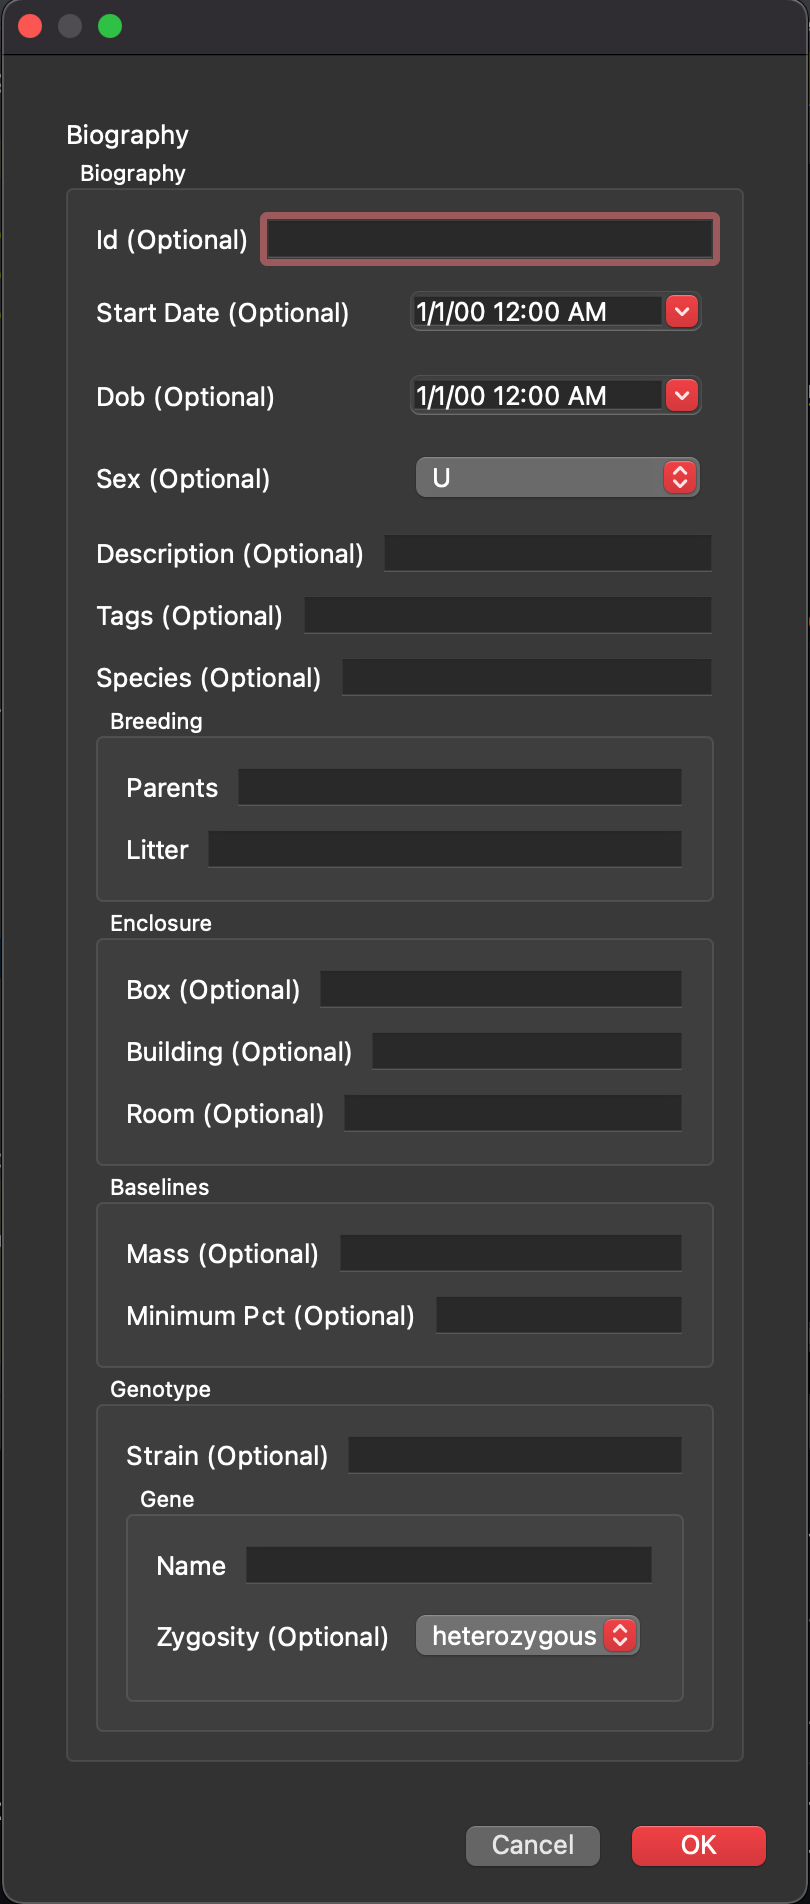
\includegraphics[width=\linewidth]{figures/model_form.png}
\caption{An Autopilot Data model can automatically generate a GUI form to fill in its properties, in this example to define a new experimental Subject's biography.}
\label{fig:modelform}
\end{marginfigure}

Though the data modeling system is new\sidenote{Released as an alpha version at the time of writing}, we have laid the groundwork for Autopilot's plugin system to allow researchers to declare custom schema for all data produced by Autopilot, and to preserve both interoperability and reproducibility by combining them with datasets potentially produced by multiple incompatible tools (see Section \ref{future:data}).



